\documentclass[a4paper,11pt]{article}

\usepackage[margin=3cm]{geometry}

\usepackage{graphicx}
\usepackage{subcaption}
\usepackage[colorlinks,allcolors=violet]{hyperref}
\usepackage{url}
\usepackage{lmodern}

% https://tex.stackexchange.com/questions/94032/fancy-tables-in-latex
\usepackage[table]{xcolor}
\usepackage{booktabs}

\usepackage[utf8]{inputenc}

% https://tex.stackexchange.com/questions/664/why-should-i-use-usepackaget1fontenc
\usepackage[T1]{fontenc}
\usepackage{microtype} % good font tricks

\newcommand{\note}[1]{{\colorbox{yellow!40!white}{#1}}}
\newcommand{\exampletext}[1]{{\color{blue!60!black}#1}}

\begin{document}

\noindent
\colorbox[HTML]{52BDEC}{\bfseries\parbox{\textwidth}{\centering\large
  --- Report P\&O CW 2019--2020 Task <tasknumber> ---
}}
\\[-1mm]
\colorbox[HTML]{00407A}{\bfseries\color{white}\parbox{\textwidth}{
  Department of Computer Science -- KU Leuven
  \hfill
  \today
}}
\\

\smallskip

\noindent
%\mbox{}\hfill
\begin{tabular}{*4l}
\toprule
\multicolumn{2}{l}{\large\textbf{Team <number>}} \\
\midrule
<team member 1> & 25h \\ % fill in the time spend on this task per team member who worked on it
<team member 2> & 15h \\
<team member 3> & 30h \\
\bottomrule
\hline
\end{tabular}\\
\\
Demo: \url{https://penocw.cs.kotnet.kuleuven.be:80##/demo-task-44?0xjwkkslam9}

\noindent
{\color[HTML]{52BDEC} \rule{\linewidth}{1mm} }

\section{Introduction}\label{sec:introduction}

\note{(Few sentences.)}
\exampletext{
\textit{Clearly state the problem you tackled. The task's assignment defined the functionality you have to offer, not the problem(s) you solved. You have to phrase the exact problem statement, i.e., state the assumptions you made. On top of the problem statement we expect you to state the relevance of the problem and what solution is chosen. Later in \S\ref{sec:technical-analysis} you can go into detail as why this is your preferred solution. Throughout the text we expect you to back up claims with (scientific) references.
\textbf{This section is best written after the remainder of the report is finished.}}}

\exampletext{
We are developing a multiscreen casting framework that supports a heterogeneous set of displays. The very first hurdle is the design of a communication protocol that connects all these devices. Devices are connected over the web via a client-server architecture. Clients connect to the server by loading a webpage in their browser. To establish a two-way communication channel, a connection is maintained through sockets~\cite{socketio}.

Based on these principles we developed a basic multiscreen casting framework that offers the following functionality:
\begin{itemize}
    \item The ability to transmit complex data such as images.
    \item Client-side access to the camera.
    \item Client identification such that clients can receive specific commands.
    \item Support of two roles, i.e., master and slave.
\end{itemize}
% The communication protocol should accommodate for:
% \begin{itemize}
%     \item The transmission of images from the smartphone camera to the master.
%     \item Manipulation of the background color of the client screens.
% \end{itemize}
% We are developing a game that requires two players who engage in a confrontation to take a mug shot picture of each other.
% Our game rules will positively encourage both players to provide clean pictures.
% This turned out to be essential since the DeepFace neural network \cite{website:facerecognizer} that we use was not accurate enough in the other scenario's we tested.
% Our analysis of the recognition rate is given in \S\ref{sec:technical-analysis}. Our systematic tests showed we have less than $1\%$~probability of not identifying the correct user out of our test database with $1000$ representative mugshot pictures.

% One unforeseen side effect of the usage of the DeepFace~\cite{amos2016openface} algorithm is the high power consumption.
% We had to balance the performance of the face recognition with battery life time. This was most significant for our indoor game play. In a test run we estimated that the average mobile phone from the supported types will be capable of playing for about $4$~hours and in that time frame scanning and identifying $60$~pictures per hour, see \S\ref{sec:technical-analysis}.
}

\section{Design schematics and screenshots}\label{sec:schematic}

\note{($\approx$ 1 page. Depending on the need for a design overview.)}
\exampletext{\textit{Design schematics, deployment diagrams, class diagrams, sequence diagrams, \ldots\ Whatever you think we need to understand your design. You could add a little bit of text here but keep that under half a page. You reference the illustrations here from~\S\ref{sec:technical-analysis} when needed.}}

\exampletext{All communication between clients runs through a nodejs server. We use the Socketio~\cite{socketio} library to set up a bidirectional communication channel between client and server. A deployment diagram can be found in Figure~\ref{fig:deployment}. Clients can take on a specific master or slave role by opening a specific webpage within the browser, i.e., the slaves will surf to \texttt{webaddress/slave}, while a client that wants to be the master loads the webpage found at \texttt{webaddress/master}.}

\begin{figure}[h!]
	\centering
	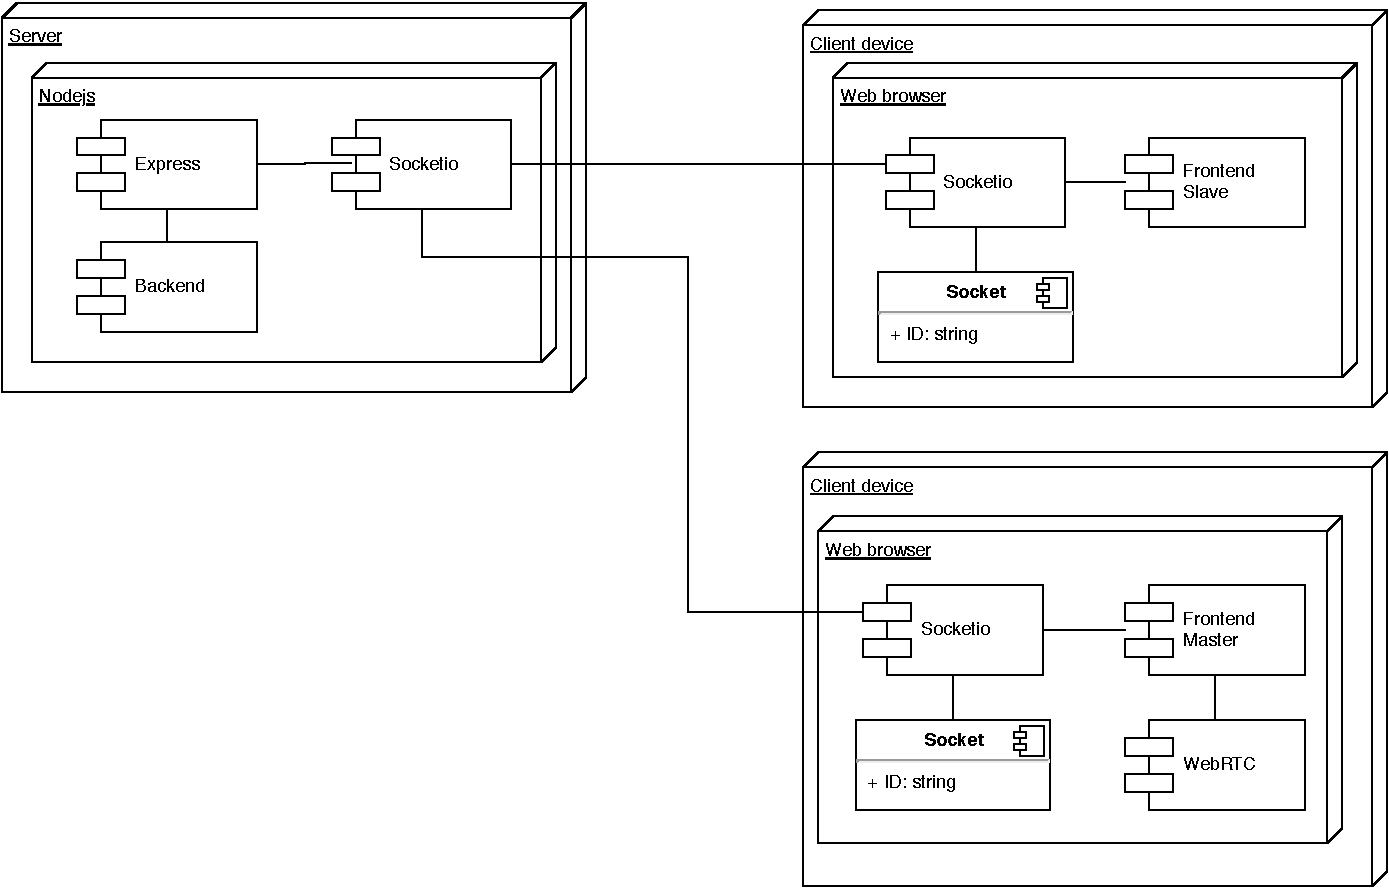
\includegraphics[width=\textwidth]{figures/deployment}
	\caption{Deployment diagram of the multiscreen casting framework.} 
	\label{fig:deployment}
\end{figure}

\exampletext{We rely on webrtc~\cite{website:webrtc} to collect a client-side video stream. This module offers the necessary tools for serialization, i.e., as a base64 encoded string. Serialization is required for transmission~\cite{website:serialization}. Server-side the backend code will process the image. In our demo we broadcast the image by sending it to all slaves. Slaves and masters can be reached by the server, as we use the concept of a namespace~\cite{website:namespaces}. A namespace can be used to group clients with a similar role, and broadcast to them. 

A socket is assigned a unique identifier by Socketio. This identifier can be used to emit messages from the server to a specific client. A list of connected clients is available through the API of Socketio \cite{website:socketio-clients}.}

\section{Algorithms}\label{sec:technical-analysis}

\note{($\approx$ 1 page. Depending on necessity)}
\exampletext{\textit{When you design or use an algorithm you should be able to explain how well it performs and if it satisfies the requirements. Often there will be alternatives or system parameters that need to be chosen. We want to know why you chose a specific set of parameters, or why you chose an approach over another. We supply some example text of last year.}}

\exampletext{
Correctly identifying players is an important requirement of the game. For this end we adapt a Face Recognition system that builds on the \texttt{facerecognizer.js} framework~\cite{website:facerecognizer}. We show that by carefully selecting hyper parameters we can assure that misidentification will happen in less than 1\% of identifications.


\subsection{Description of the face recognition system}

We illustrate the face recognition pipeline in Figure~\ref{fig:identification}. This pipeline is fully offered by the \texttt{facerecognizer.js} framework~\cite{website:facerecognizer}. However, since we have only one enrollment sample, we will only use the core technology of the framework, i.e., DeepFace~\cite{amos2016openface}, the feature extractor method. Deepface represents the face image as a 128 dimensional vector with values in the interval $[-1,1]$. In a second step a similarity score is calculated between the enrollment samples of all known identities and the test sample. For this end, we evaluate the impact of two similarity metrics on the performance: \texttt{profnuyenssimilarity}~\cite{nuyens:2018} and \texttt{profjacobsdistance}~\cite{jacobs:2015} in \S\ref{sec:experimenten}. In a last step the highest score is compared to a threshold. If the highest score is bigger then the threshold we return the identity connected to this score, else we conclude that the test subject is unknown. The two mentioned metrics can both be formulated by
\[
  S(a, b)
  =
  \sqrt{
    \int_0^1 \int_0^1
      \|\mathcal{P}_\nu(a, t_1, t_2) - \mathcal{P}_\nu(b, t_1, t_2)\|_{\mathcal{F}}^2
      \, \mathrm{d}t_1 \mathrm{d}t_2
  }
  ,
\]
where $\mathcal{P}$ is a polynomial interpolation operator.

\begin{figure}
	\centering
	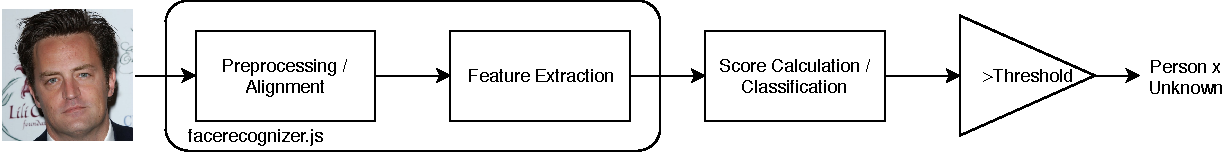
\includegraphics[width=\textwidth]{figures/identification}
	\caption{The face recognition pipeline. Face image from \textsf{lfw} data set~\cite{LFWTech}.} 
	\label{fig:identification}
\end{figure}

\subsection{Data set}

Representative data is needed to test the performance of a machine learning system. We evaluated our system in a first phase with a standard data set, i.e., labeled face in the wild~\cite{LFWTech}. This data set contains $10340$ identities with approximately 5 images per identity.

\subsection{Experiments}\label{sec:experimenten}

We discuss the influence the performance of our identification system in function of two similarity functions: \texttt{profnuyenssimilarity}~\cite{nuyens:2018} and \texttt{profjacobsdistance}~\cite{jacobs:2015}. The performance is measured in \texttt{adalbertoscore}~\cite{vanhamme:1991}. In order to achieve the requirement of a misidentification probability of $1$\%, \texttt{adalbertoscore} should be less then $-4$.

We calculate the feature vector of all the faces in \textsf{lfw}. Then, we split the data set in a enrollment and test set. We make sure that only for enrollment only one sample is available for each identity. We repeat this split procedure $10$ times and report the average score. For every split we evaluate the performance in function of the threshold. Figure~\ref{fig:performance} shows \texttt{adalbertoscore} for both similarity functions w.r.t.\ the threshold. We chose the \texttt{profnuyenssimilarity} as this clearly satisfies the requirement of a \texttt{adalbertoscore} of $-10$ at a threshold of $0.5$.
We note however that the \texttt{profnuyenssimilarity} needs a resolution of at least $5$MP which is currently not a problem, but might be a concern in the later development such that we keep the \texttt{profjacobsdistance} implementation as an alternative.

\begin{figure}
\centering
\begin{minipage}[b]{.43\textwidth}
	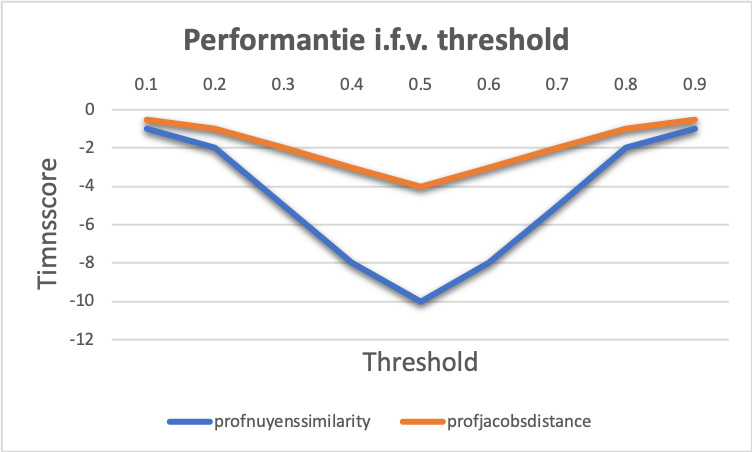
\includegraphics[width=\linewidth]{figures/performance}
	\caption{The \texttt{adalbertoscore} for both the \texttt{profnuyenssimilarity} and \texttt{profjacobsdistance} w.r.t.\ the threshold. The number of classes is $10350$.} 
	\label{fig:performance}
\end{minipage}
\hspace{1cm}
\begin{minipage}[b]{.43\textwidth}
	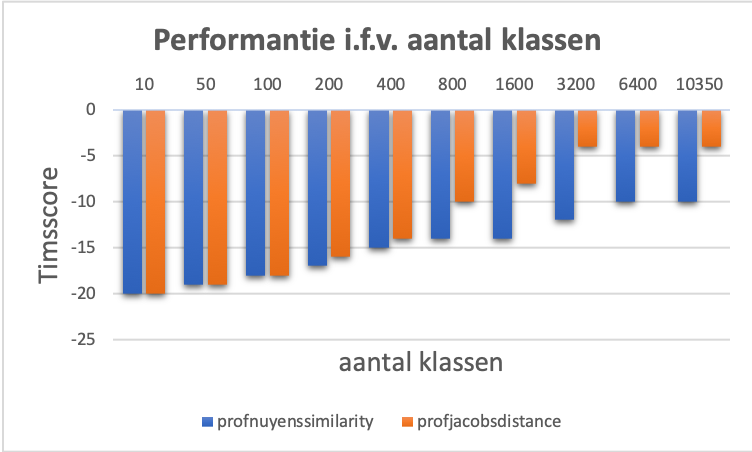
\includegraphics[width=\linewidth]{figures/performanceClasses}
	\caption{The performance w.r.t.\ the number of classes for both the \texttt{profnuyenssimilarity} and \texttt{profjacobsdistance}. The threshold is $0.5$.} 
	\label{fig:performanceClasses}
\end{minipage}
\end{figure}

In a second experiment we vary the number of classes. We fix the threshold to $0.5$. Before make the enrollment and test splits we randomly select a specific number of identities. Afterwards we apply the same procedure as in the first experiment. The results are shown in Figure~\ref{fig:performanceClasses}. From this figure we conclude that, in general the identification performance is better with a lower number of players. On top of that, when the number of players is less then $200$, both similarity functions perform similar.

In a third experiment we investigated the battery consumption\ldots
}

\section{Conclusion and prospects}\label{sec:conclusion}

\note{($\approx$ 1/4 page.)}
\exampletext{\textit{This section contains your evaluation of the development. How well did you succeed to complete this task? What can be improved?}}

\exampletext{We designed a basic framework for screen casting. We offer all the functionality demanded in task 2. We achieved our goal by relying on basic socket.io functionality, as well as built-in features of front facing html5 technology such as webrtc. We did not discuss in detail the sending of commands to change background colors etc. We offer all functionality for this problem, the core challenge here was socket identification.

In the current state of our project multiple masters can coexist. We do not see this as a problem at the moment. From a security perspective this can be problematic depending on the actual usage scenario of the final application.}


%%%%%%%%%%%%%%%%%%%%%%%%%%%%%%%%%%%%%%
%%%%%%%%%%%%%%%%%%%%%%%%%%%%%%%%%%%%%%
\appendix

%%%%%%%%%%%%%%%%%%%%%%%%%%%%%%%%%%%%%%
\section{User licenses}

\exampletext{\textit{For every software package and all images/illustrations/pictures used we want to see that you have looked up its user license and comply with it. Please provide a list here. This may also be a good location to write about what software license you are thinking for your finished project.}}

%%%%%%%%%%%%%%%%%%%%%%%%%%%%%%%%%%%%%%
\bibliographystyle{plain}
\bibliography{bibliography}

% \bigskip

% \vspace*{\fill}

% %% This is a basic score card
% %% please fill in your team number and name
% %% don't touch the rest!
% %%%%%%%%%%%%%%%%%%%%%%%%%%%%%%%%%%%%%%
% \noindent
% %\mbox{}\hfill
% \begin{tabular}{*3l}
% \toprule
% \multicolumn{3}{l}{\large\textbf{Evaluation card: Team <number> <name>}} \\
% Criterion & Score (/10) & Remarks \hspace{6cm} \\
% \midrule
% References \\
% Algorithm descriptions \\
% Correctness \\
% Clearness \\
% Writing style \\
% Conciseness \\
% Self-evaluation \\
% Informative figures \\
% Tests \\
% \bottomrule
% \hline
% \end{tabular}

\end{document}